\documentclass[12pt, a4paper]{article}

% ── Packages ──────────────────────────────────────────────────────
\usepackage[utf8]{inputenc}
\usepackage[T1]{fontenc}
\usepackage{amsmath, amssymb, amsthm}
\usepackage{mathtools}
\usepackage{enumitem}
\usepackage{tikz}
\usetikzlibrary{calc, positioning, arrows.meta, fit, patterns, decorations.pathreplacing}
\usepackage{geometry}
\geometry{margin=2.4cm}
\usepackage{xcolor}
\usepackage{tcolorbox}
\tcbuselibrary{theorems, skins, breakable}
\usepackage{booktabs}
\usepackage{hyperref}
\hypersetup{colorlinks=true, linkcolor=blue!60!black, urlcolor=blue!60!black}

\setlength{\parindent}{0pt}
\setlength{\parskip}{6pt}

% ── Colours ───────────────────────────────────────────────────────
\definecolor{setA}{RGB}{66, 133, 244}   % blue
\definecolor{setB}{RGB}{234, 67, 53}    % red
\definecolor{setC}{RGB}{251, 188, 4}    % yellow
\definecolor{theoryBg}{RGB}{232, 245, 253}
\definecolor{theoryFrame}{RGB}{66, 133, 244}
\definecolor{stmtBg}{RGB}{255, 243, 224}
\definecolor{stmtFrame}{RGB}{230, 126, 34}
\definecolor{ansBg}{RGB}{232, 250, 232}
\definecolor{ansFrame}{RGB}{39, 174, 96}

% ── Environments ──────────────────────────────────────────────────
\newtcolorbox{theorybox}[1][]{%
  colback=theoryBg, colframe=theoryFrame,
  fonttitle=\bfseries, title={\small Theory Recap: #1},
  breakable, enhanced, arc=2mm,
  left=5pt, right=5pt, top=5pt, bottom=5pt
}

\newtcolorbox{problembox}{%
  colback=stmtBg, colframe=stmtFrame,
  fonttitle=\bfseries, title={\small Problem Statement},
  breakable, enhanced, arc=2mm,
  left=5pt, right=5pt, top=5pt, bottom=5pt
}

\newtcolorbox{answerbox}{%
  colback=ansBg, colframe=ansFrame,
  arc=2mm, left=5pt, right=5pt, top=3pt, bottom=3pt
}

\newcommand{\Z}{\mathbb{Z}}
\newcommand{\R}{\mathbb{R}}
\newcommand{\N}{\mathbb{N}}
\newcommand{\powset}[1]{2^{#1}}
\newcommand{\comp}[1]{\overline{#1}}
\newcommand{\symdiff}{\mathbin{\triangle}}

% ── Title ─────────────────────────────────────────────────────────
\title{\textbf{Practice 8 --- Recurrence Relations}\\[4pt]
       \large Solutions to Selected Problems\\[2pt]
       \normalsize Problems 2, 6}
\author{Discrete Mathematics --- QYSU}
\date{}

\begin{document}
\maketitle
\tableofcontents
\newpage

% ══════════════════════════════════════════════════════════════════
\section{Problem 2 --- Solving a Second-Order Linear Recurrence}
% ══════════════════════════════════════════════════════════════════

\begin{theorybox}[Second-Order Linear Recurrences with Constant Coefficients]
A \textbf{second-order linear recurrence with constant coefficients} has the form
\[
  a_n = c_1\, a_{n-1} + c_2\, a_{n-2}, \qquad n \ge 2,
\]
where $c_1, c_2$ are constants and $a_0, a_1$ (or $a_1, a_2$) are given initial values.

\medskip
\textbf{The Characteristic Equation Method.}\;
Substitute the trial solution $a_n = r^n$ into the recurrence to obtain the
\textbf{characteristic equation}:
\[
  r^2 - c_1\, r - c_2 = 0.
\]

The form of the general solution depends on the roots $r_1, r_2$:

\medskip
\begin{center}
\renewcommand{\arraystretch}{1.5}
\begin{tabular}{lll}
\toprule
\textbf{Case} & \textbf{Roots} & \textbf{General Solution} \\
\midrule
Distinct real roots & $r_1 \neq r_2$, both real
  & $a_n = \alpha\, r_1^n + \beta\, r_2^n$ \\
Repeated real root & $r_1 = r_2 = r$
  & $a_n = (\alpha + \beta\, n)\, r^n$ \\
Complex conjugate roots & $r_{1,2} = \rho\, e^{\pm i\theta}$
  & $a_n = \rho^n\bigl(\alpha \cos n\theta + \beta \sin n\theta\bigr)$ \\
\bottomrule
\end{tabular}
\end{center}

\medskip
The constants $\alpha$ and $\beta$ are determined by substituting the initial conditions
into the general solution and solving the resulting $2 \times 2$ linear system.

\begin{center}
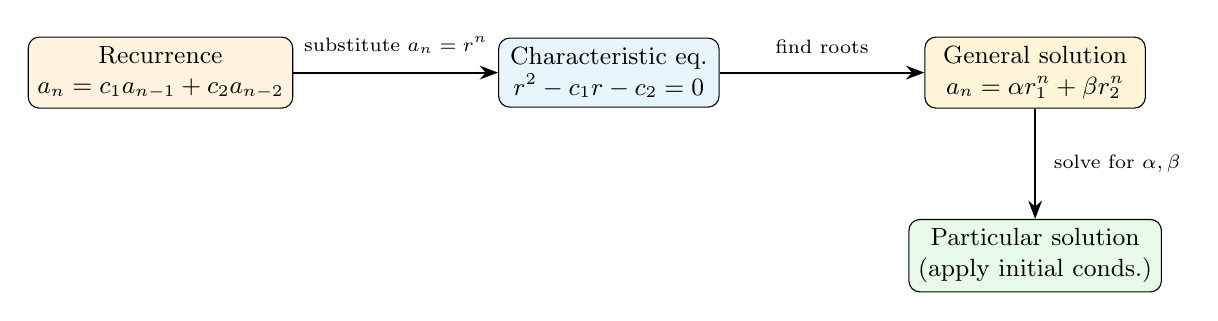
\begin{tikzpicture}[>=Stealth, font=\small, node distance=1.6cm]
  \node[draw, rounded corners=4pt, fill=stmtBg, minimum width=2.8cm,
        align=center, font=\small] (rec) {Recurrence\\$a_n = c_1 a_{n-1} + c_2 a_{n-2}$};
  \node[draw, rounded corners=4pt, fill=theoryBg, minimum width=2.8cm,
        align=center, font=\small, right=2.6cm of rec] (char)
    {Characteristic eq.\\$r^2 - c_1 r - c_2 = 0$};
  \node[draw, rounded corners=4pt, fill=setC!15, minimum width=2.8cm,
        align=center, font=\small, right=2.6cm of char] (gen)
    {General solution\\$a_n = \alpha r_1^n + \beta r_2^n$};
  \node[draw, rounded corners=4pt, fill=ansBg, minimum width=2.8cm,
        align=center, font=\small, below=1.4cm of gen] (sol)
    {Particular solution\\(apply initial conds.)};

  \draw[->, thick] (rec) -- (char)
    node[midway, above=3pt, font=\scriptsize]{substitute $a_n = r^n$};
  \draw[->, thick] (char) -- (gen)
    node[midway, above=3pt, font=\scriptsize]{find roots};
  \draw[->, thick] (gen) -- (sol)
    node[midway, right=3pt, font=\scriptsize]{solve for $\alpha, \beta$};
\end{tikzpicture}
\end{center}
\end{theorybox}

\begin{problembox}
Solve the linear recurrence relation
\[
  a_n = 5a_{n-1} - 6a_{n-2}, \qquad n > 2,
\]
with initial conditions $a_1 = 2$ and $a_2 = 10$.
\end{problembox}

\subsection*{Solution}

\textbf{Step 1: Write the characteristic equation.}

The recurrence $a_n - 5a_{n-1} + 6a_{n-2} = 0$ has characteristic equation
\[
  r^2 - 5r + 6 = 0.
\]

\textbf{Step 2: Find the roots.}

Factoring:
\[
  r^2 - 5r + 6 = (r - 2)(r - 3) = 0
  \qquad\Longrightarrow\qquad r_1 = 2, \quad r_2 = 3.
\]
The roots are distinct and real, so we are in \textbf{Case 1}.

\begin{center}
\begin{tikzpicture}[>=Stealth, font=\small]
  % Parabola for r^2 - 5r + 6
  \draw[->, thick] (-0.5, 0) -- (5.5, 0) node[right]{$r$};
  \draw[->, thick] (0, -1.5) -- (0, 4) node[above]{$r^2 - 5r + 6$};

  \draw[thick, setA, domain=0.5:4.5, samples=60]
    plot (\x, {(\x - 2)*(\x - 3)});

  % Roots
  \fill[setB] (2, 0) circle (3pt) node[below left=3pt, font=\footnotesize]{$r_1 = 2$};
  \fill[setB] (3, 0) circle (3pt) node[below right=3pt, font=\footnotesize]{$r_2 = 3$};

  % Tick marks
  \foreach \x in {1, 2, 3, 4} {
    \draw (\x, 0.08) -- (\x, -0.08);
  }
  \node[below, font=\tiny] at (1, -0.08) {$1$};
  \node[below, font=\tiny] at (4, -0.08) {$4$};
\end{tikzpicture}
\end{center}

\textbf{Step 3: Write the general solution.}

Since $r_1 = 2$ and $r_2 = 3$ are distinct real roots:
\[
  a_n = \alpha \cdot 2^n + \beta \cdot 3^n.
\]

\textbf{Step 4: Apply initial conditions.}

Substituting $n = 1$ and $n = 2$:
\[
  \begin{cases}
    a_1 = 2\alpha + 3\beta = 2 \\[3pt]
    a_2 = 4\alpha + 9\beta = 10
  \end{cases}
\]

From the first equation:
\[
  \alpha = \frac{2 - 3\beta}{2} = 1 - \frac{3\beta}{2}.
\]

Substituting into the second equation:
\[
  4\!\left(1 - \frac{3\beta}{2}\right) + 9\beta = 10
  \quad\Longrightarrow\quad
  4 - 6\beta + 9\beta = 10
  \quad\Longrightarrow\quad
  3\beta = 6
  \quad\Longrightarrow\quad
  \beta = 2.
\]

Then $\alpha = 1 - \dfrac{3 \cdot 2}{2} = 1 - 3 = -2$.

\textbf{Step 5: Write the particular solution.}

\[
  a_n = -2 \cdot 2^n + 2 \cdot 3^n = 2\bigl(3^n - 2^n\bigr).
\]

\textbf{Step 6: Verify.}

\begin{center}
\renewcommand{\arraystretch}{1.3}
\begin{tabular}{cccc}
\toprule
$n$ & $2(3^n - 2^n)$ & Expected & Match \\
\midrule
$1$ & $2(3 - 2) = 2$ & $a_1 = 2$ & $\checkmark$ \\
$2$ & $2(9 - 4) = 10$ & $a_2 = 10$ & $\checkmark$ \\
$3$ & $2(27 - 8) = 38$ & $5(10) - 6(2) = 38$ & $\checkmark$ \\
$4$ & $2(81 - 16) = 130$ & $5(38) - 6(10) = 130$ & $\checkmark$ \\
\bottomrule
\end{tabular}
\end{center}

\begin{answerbox}
\centering
$a_n = 2\bigl(3^n - 2^n\bigr)$
\end{answerbox}

% ══════════════════════════════════════════════════════════════════
\newpage
\section{Problem 6 --- Binary Strings with Two Consecutive Zeros}
% ══════════════════════════════════════════════════════════════════

\begin{theorybox}[Complementary Counting and Recurrences for Constrained Strings]
\textbf{Complementary counting.}\;
When counting objects that satisfy a property $P$, it is sometimes easier
to count those that do \emph{not} satisfy $P$:
\[
  |P| = |\text{total}| - |\text{not } P|.
\]

\textbf{Setting up recurrences for constrained strings.}\;
To count binary strings of length $n$ satisfying (or avoiding) a pattern:
\begin{enumerate}[nosep]
  \item Define a sequence: let $b_n$ be the count of valid strings of length~$n$.
  \item \textbf{Condition on the first (or last) character.}\;
        Each choice constrains what can follow, yielding a recurrence.
  \item Solve using base cases.
\end{enumerate}

\medskip
\textbf{Example pattern: avoiding ``$00$''.}\;
For a string of length $n$ with no two consecutive $0$s:
\begin{itemize}[nosep]
  \item If it starts with \texttt{1}: the remaining $n-1$ characters form any valid
        string $\longrightarrow$ $b_{n-1}$ choices.
  \item If it starts with \texttt{0}: the next character \emph{must} be \texttt{1}
        (to avoid ``$00$''), and the remaining $n-2$ characters form any valid
        string $\longrightarrow$ $b_{n-2}$ choices.
\end{itemize}
This gives the Fibonacci-like recurrence $b_n = b_{n-1} + b_{n-2}$.

\begin{center}
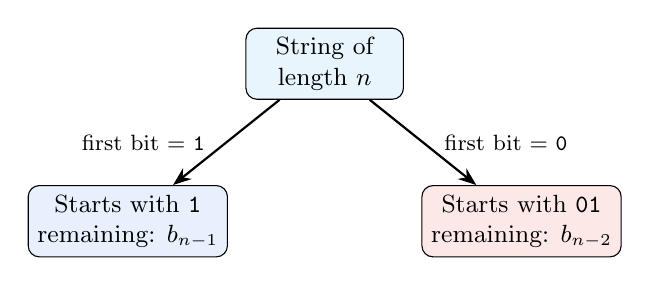
\begin{tikzpicture}[>=Stealth, font=\small,
  level distance=2.0cm, sibling distance=5.0cm,
  edge from parent/.style={draw, thick, ->, >=Stealth},
  every node/.style={align=center}]
  \node[draw, rounded corners, fill=theoryBg, minimum width=2.0cm]
    {String of\\length $n$}
    child {
      node[draw, rounded corners, fill=setA!12, minimum width=2.0cm]
        {Starts with \texttt{1}\\remaining: $b_{n-1}$}
      edge from parent node[left=4pt, font=\footnotesize] {first bit = \texttt{1}}
    }
    child {
      node[draw, rounded corners, fill=setB!12, minimum width=2.0cm]
        {Starts with \texttt{01}\\remaining: $b_{n-2}$}
      edge from parent node[right=4pt, font=\footnotesize] {first bit = \texttt{0}}
    };
\end{tikzpicture}
\end{center}
\end{theorybox}

\begin{problembox}
How many binary strings of length 10 contain two consecutive zeros?
\end{problembox}

\subsection*{Solution}

We use \textbf{complementary counting}.

\textbf{Step 1: Count all binary strings of length 10.}

Each position has 2 choices, so the total is $2^{10} = 1024$.

\textbf{Step 2: Count binary strings of length 10 with \emph{no} two consecutive zeros.}

Let $b_n$ denote the number of binary strings of length $n$ with no two
consecutive $0$s.

\textbf{Deriving the recurrence.}\;
Consider a valid string of length $n$:
\begin{itemize}[nosep]
  \item If it starts with \texttt{1}: the remaining $n-1$ characters can be
        any valid string of length $n-1$, giving $b_{n-1}$ choices.
  \item If it starts with \texttt{0}: the next character must be \texttt{1}
        (otherwise we have ``$00$''), and the remaining $n-2$ characters can be
        any valid string of length $n-2$, giving $b_{n-2}$ choices.
\end{itemize}

Therefore:
\[
  b_n = b_{n-1} + b_{n-2}, \qquad n \ge 3.
\]

\textbf{Base cases.}
\begin{itemize}[nosep]
  \item $b_1 = 2$: the strings are \texttt{0} and \texttt{1}.
  \item $b_2 = 3$: the valid strings are \texttt{01}, \texttt{10}, \texttt{11}
        (excluding \texttt{00}).
\end{itemize}

\textbf{Step 3: Compute $b_n$ for $n = 3, 4, \ldots, 10$.}

\begin{center}
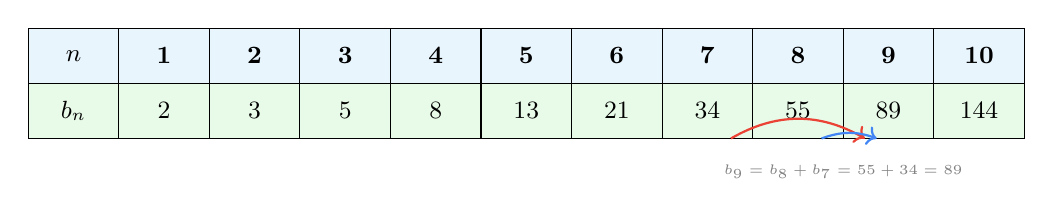
\begin{tikzpicture}[font=\small]
  % Table as a TikZ figure with colored cells
  \def\cellw{1.15}
  \def\cellh{0.7}

  % Header row
  \foreach \i/\lab in {0/$n$, 1/1, 2/2, 3/3, 4/4, 5/5, 6/6, 7/7, 8/8, 9/9, 10/10} {
    \node[draw, minimum width=\cellw cm, minimum height=\cellh cm,
          fill=theoryBg, font=\small\bfseries] at (\i*\cellw, 0) {\lab};
  }

  % Value row
  \foreach \i/\val in {0/$b_n$, 1/2, 2/3, 3/5, 4/8, 5/13, 6/21, 7/34, 8/55, 9/89, 10/144} {
    \node[draw, minimum width=\cellw cm, minimum height=\cellh cm,
          fill=ansBg, font=\small] at (\i*\cellw, -\cellh) {\val};
  }

  % Arrows showing the recurrence for one example
  \draw[->, thick, setB, bend left=30]
    (7*\cellw + 0.3, -\cellh - 0.35) to
    node[below, font=\tiny, setB!70!black] {}
    (9*\cellw - 0.3, -\cellh - 0.35);
  \draw[->, thick, setA, bend left=20]
    (8*\cellw + 0.3, -\cellh - 0.35) to
    node[below, font=\tiny] {}
    (9*\cellw - 0.15, -\cellh - 0.35);

  \node[font=\tiny, gray] at (8.5*\cellw, -2.1*\cellh)
    {$b_9 = b_8 + b_7 = 55 + 34 = 89$};
\end{tikzpicture}
\end{center}

Detailed computation:
\begin{alignat*}{3}
  b_3 &= b_2 + b_1 &&= 3 + 2 &&= 5 \\
  b_4 &= b_3 + b_2 &&= 5 + 3 &&= 8 \\
  b_5 &= b_4 + b_3 &&= 8 + 5 &&= 13 \\
  b_6 &= b_5 + b_4 &&= 13 + 8 &&= 21 \\
  b_7 &= b_6 + b_5 &&= 21 + 13 &&= 34 \\
  b_8 &= b_7 + b_6 &&= 34 + 21 &&= 55 \\
  b_9 &= b_8 + b_7 &&= 55 + 34 &&= 89 \\
  b_{10} &= b_9 + b_8 &&= 89 + 55 &&= 144
\end{alignat*}

\textbf{Observation.}\; The values $b_n = 2, 3, 5, 8, 13, 21, 34, 55, 89, 144$
are the Fibonacci numbers $F_3, F_4, \ldots, F_{12}$.
In general, $b_n = F_{n+2}$ where $F_1 = 1, F_2 = 1, F_3 = 2, \ldots$

\textbf{Step 4: Apply complementary counting.}

\[
  \text{Strings with ``$00$''} = \text{Total} - \text{Strings without ``$00$''}
  = 1024 - 144 = 880.
\]

\textbf{Verification for small cases.}\;
For $n = 2$: total $= 4$, strings without ``$00$'' $= 3$ (\texttt{01, 10, 11}),
so strings with ``$00$'' $= 1$ (namely \texttt{00}). \checkmark

For $n = 3$: total $= 8$, $b_3 = 5$ (\texttt{010, 011, 101, 110, 111}),
so strings with ``$00$'' $= 3$ (\texttt{001, 100, 000}). \checkmark

\begin{answerbox}
\centering
The number of binary strings of length 10 that contain two consecutive zeros is
$\boxed{880}$.
\end{answerbox}

\end{document}
